\begin{figure*}
\centering
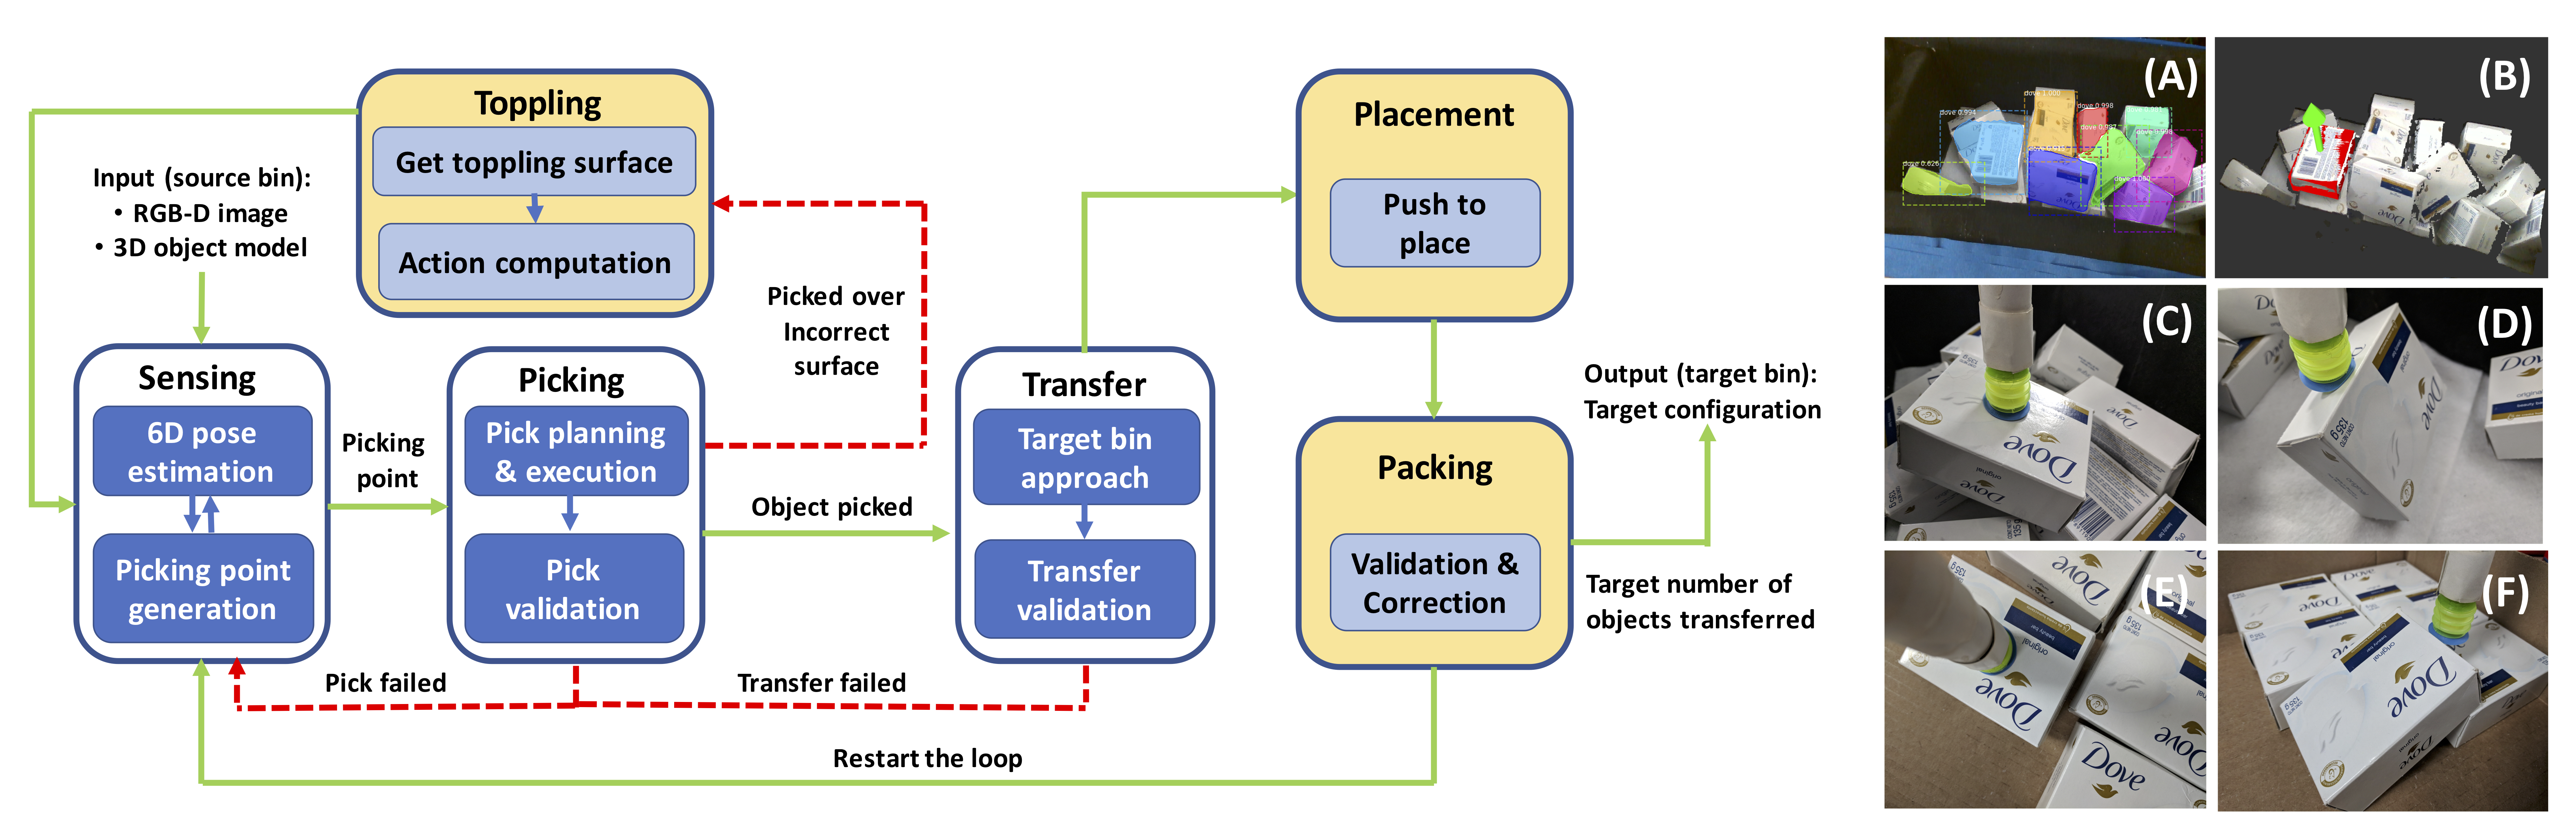
\includegraphics[width=1\textwidth]{Figures/final_pipeline.png}
\vspace{-0.1in}
\caption{\textit{Left}: Pipeline in terms of control, data flow (green lines) and failure handling (red lines). The blocks identify the modules of the system. Sensing receives an RGBD image of $\binit$ and object CAD models to return a grasp point. Based on the picking surface, the object is either transferred to $\btarget$ or is handled by the {\tt Toppling} module, which flips the object and places it back in $\binit$. When the object is transferred, a robust {\tt Placement} module places the object at the target pose $\hat{p}^i$. The Packing module validates and corrects the placement to achieve tight packing. \textit{Right}: a) Instance segmentation. b) Pose estimation and picking point selection are provided by sensing, c) Picking d) Toppling e) Placement and f) Packing.
}
\vspace{-0.2in}
\label{fig:pipeline}
\end{figure*}

Consider a robotic arm in a workspace $\Wspace$ with known static obstacles, two bins $\binit$ and $\btarget$, as well as $n$ movable, uniform objects $\objectset=\{ \object^1, \ldots, \object^n \}$ of known cubic dimensions. The bins $\binit$ and $\btarget$ are static but also compliant bodies in known poses that define a cuboid volume in $\Wspace$ where the objects can be placed. 

A labeled arrangement $\arrangement = \{ \pose^1, \ldots, \pose^n \}$ is an assignment of poses $\pose^i \in SE(3)$ to each object $\object^i$. Initially, the objects are in a start arrangement $\ainit$, where the objects are inside $\binit$ in random but ``stable'' poses, i.e., the objects are stably resting and not moving. The $\ainit$ arrangement is \emph{not} known a-priori to the robot. 

The objective is to move $\objectset$ to an unlabeled arrangement $\atarget = \{ \hat{\pose}^1, \ldots, \hat{\pose}^n \}$, which achieves a tight packing in $\btarget$. $\atarget$ depends on the pose of $\btarget$, its dimensions and the object dimensions. The target arrangement and the picking order is input for the proposed process. The target arrangement maximizes the number of objects inside  $\btarget$, while the objects rest on a stable face, and minimizes the convex hull of the volume the objects $\objectset$ occupy in $\Wspace$. This is typically a grid-like regular packing for cuboid objects. The unlabeled nature of $\atarget$ means it is satisfied as long as one of the objects is placed at each target pose, i.e.,

\vspace*{-5mm}
\begin{equation}
\forall \hat{\pose}^j \in \atarget: \exists\  \object^i \in \objectset \textrm{ so that } D(\hat{\pose}^j, p^i) < \epsilon,
\label{eq:satisfaction}
\end{equation}

\noindent where $\epsilon$ is a threshold for achieving the target poses; $D(\cdot,\cdot)$ is distance between object poses, which should consider the 3-axis symmetry of the cubic objects. In particular, if two poses result into an object occupying the same volume, then their distance is 0. For instance, rotation by $\pi$ about the vertical axis for a stably resting cube on a flat surface results in distance 0. A popular distance metric for 6D poses is the ADI metric ~\cite{hinterstoisser2012model}. The evaluation section will describe the distance used in the experimental process for evaluating the error of the final arrangement given point cloud data.

%, i.e., any rotation by $\pi$ about any axis perpendicular to an object surface that goes through its center results in the same volume being occupied. The experimental section will provide more details on the evaluation of this distance function given sensing data.   

%, where  $\cfull$ is the space of all possible arm configurations $q \in \cfull$

The arm has $d$ joints that define the arm's configuration space $\cfull \subset \mathbb{R}^d$, which has a collision-free subset $\cfree$. Valid arm motions correspond to a continuous C-space curve $\pi : [0,1] \rightarrow \cfree$.  The arm has an end-effector, such as a suction cup, for which discrete operations $\{ \mathtt{pick}, \mathtt{release} \}$ give rise to discrete modes: $\mathcal{M} = \{ \mathtt{transfer}, \mathtt{transit} \}$. No within hand manipulation operations are available. The state space of the arm is: $\mathcal{X} = \cfree \times \mathcal{M}$. Sensing is used to reason about the current object poses. Overall, the robot operations involve (i) moving the joints, (ii) picking or releasing objects and (iii) sensing.

%technology $S: \Wspace \rightarrow \mathcal{I}$, such as {\tt RGB-D} cameras, that can generate a representation  $\mathcal{I}$ of the workspace $\Wspace$, such as images, that allow 

The arm's forward kinematics define a mapping $\fk: \cfull \rightarrow SE(3)$, which provides the pose $g \in SE(3)$ of the end-effector given $q \in \cfull$. The reachable task space defines the end-effector poses the arm can reach without collisions: $\mathcal{T} = \{ \forall\ q \in \cfree: FK(q) \in SE(3)\}.$ For the arm to pick $\object^i$ at $\pose^i$, it has to be that the arm's end-effector pose $\grasp$ satisfies a binary output function: $\mathtt{is\_pick\_feasible}( \object^i, \pose^i, \grasp), \textrm{ where } \grasp \in \mathcal{T}.$ For instance, the pose $\grasp$ of a suction cup must align it with at least one of the surfaces of an object $\object^i$ at $\pose^i$. Then, it is possible to define the set of end-effector poses, which allow to pick an object at a specific pose: $$\graspset( \object^i, \pose^i ) = \{\grasp \in \mathcal{T}:  {\mathtt{is\_pick\_feasible}}(\object^i, \pose^i, \grasp) = true\}.$$ 

Assume the sets $\graspset( \object_i, \pose_i )$ are non-empty for all objects $\objectset$ and poses in $\ainit$ or $\atarget$ (and their vicinity inside bins $\binit$ and $\btarget$). Otherwise, the task is not feasible. Note that it may be necessary to reconfigure the objects inside the initial bin so as to pick them from the appropriate face before placing them. This is due to the lack of within-hand manipulation.

Given the above definitions, the task is to identify a sequence of motions for the arm as well as end-effector and sensing operations to transfer the objects  $\objectset$ from the unknown initial stable arrangement $\ainit$ inside $\binit$ to a tight, grid-based packing inside $\btarget$ defined by an unlabeled arrangement $\atarget$, so as to satisfy Eq. \ref{eq:satisfaction}.  